\documentclass[a4paper,11pt]{article}
\usepackage[utf8]{inputenc}
\usepackage[T1]{fontenc}
\usepackage[english]{babel}
\usepackage{times}
\usepackage{graphicx}
\textwidth=6in
\textheight=9.0in
\headheight=0in
\headsep=0in
\oddsidemargin=0in
\evensidemargin=0in
\title{SSM2164 SVF}
\author{Olivier Gillet -- \tt ol.gillet@gmail.com}
\date{}
\begin{document}

\maketitle

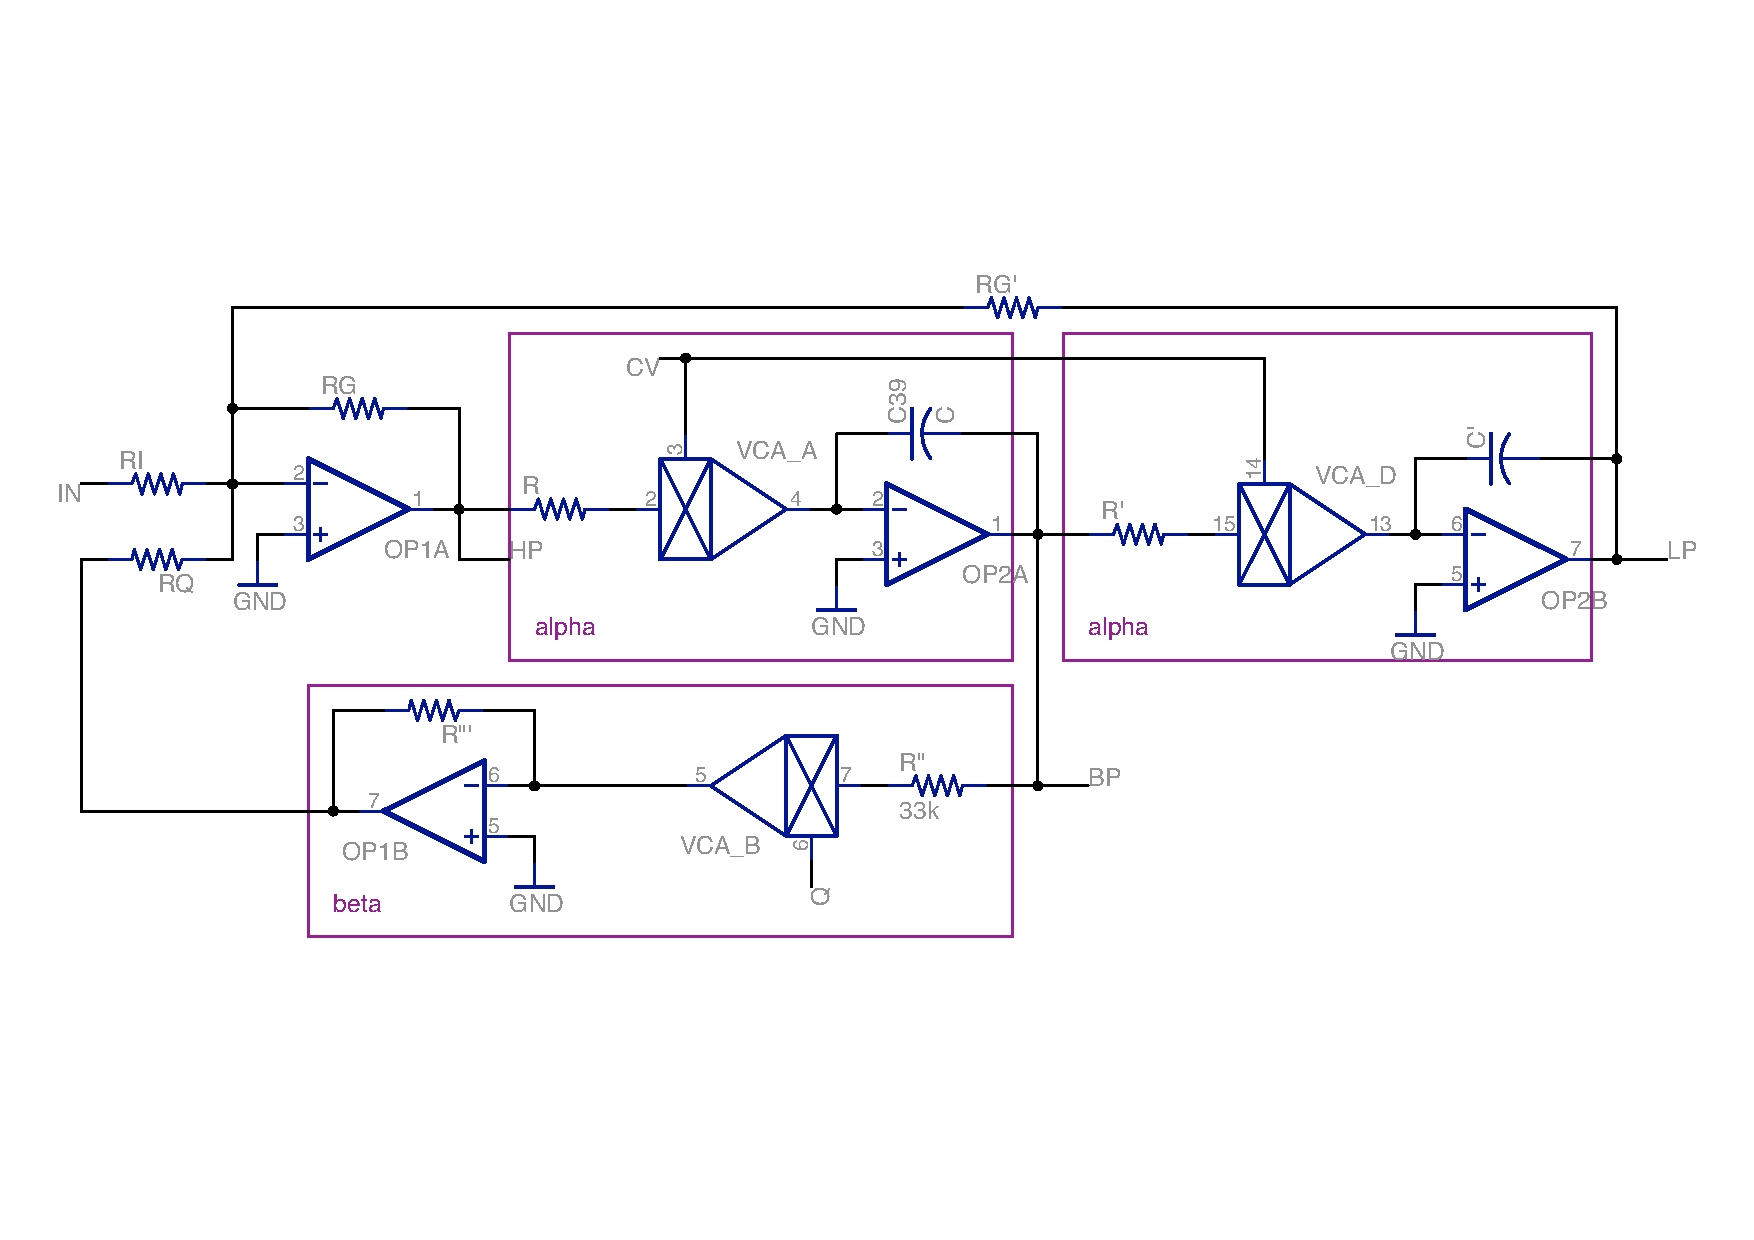
\includegraphics[width=\textwidth]{svf_schematics.pdf}

\section{Theory}

Notations:

$R_i$ is the value of the resistor through which the input signal is fed to the circuit.

$R_g$ is the value of the resistors through which the HP and LP output are fed back into the input.

$R_q$ is the value of the resistor through which the attenuated BP output is fed back into the input.

$R$ is the value of the resistors through which input voltages are converted into currents at the input of the 2164s, and through which the current at the output of the Q attenuator is converted back into a voltage.

$C$ is the value of the integrators' capacitors.

$v_{cv}$ is the cutoff frequency control voltage and $v_{q}$ is the Q control voltage.


The input voltage is $v_i(s)(s)$. $v_{lp}(s)$, $v_{hp}(s)$, $v_{bp}(s)$ are respectively the voltages at the low-pass, high-pass and band-pass nodes of this circuit.

As a reminder, the transfer function of a SSM2164 gain cell is $i_{out} = i_{in} 10^{-\frac{3}{2} v_{cv}}$. The transfer function of an integrator cell $\alpha$ is thus the following:

\begin{equation}
\alpha(s) = -\frac{1}{RCs} 10^{-\frac{3}{2} v_{cv}}
\end{equation}

Thus: $v_{bp}(s) = v_{hp}(s) \alpha(s)$, and $v_{lp}(s) = v_{hp}(s) \alpha^2(s)$.

The gain of the feedback circuit is noted $\beta$:

\begin{equation}
\beta = \frac{1}{R} 10^{-\frac{3}{2} v_{q}} \times -R = -10^{-\frac{3}{2} v_{q}}
\end{equation}

Since the op-amp has a huge input impedance, we can assume that the current flowing into $i^-$ is null:

\begin{equation}
\frac{v_i(s) - v^-}{R_i} + \frac{v_{hp}(s) - v^-}{R_g} + \frac{v_{lp}(s) - v^-}{R_g} + \frac{v_{lp}(s) - v^-}{R_g} + \frac{v_{bp}(s) \beta - v^-}{R_q} = i^- = 0
\end{equation}


The voltages at the inputs of the op-amp being equal, $v^-(s) = v^+(s) = 0$, hence:

\begin{equation}
\frac{v_i(s)}{R_i} + \frac{v_{hp}(s)}{R_g} + \frac{\alpha^2(s) v_{hp}(s)}{R_g} + \frac{v_{hp}(s) \alpha(s) \beta}{R_q} = 0
\end{equation}

The transfer function for the HP mode can be deduced from there:

\begin{eqnarray}
H_{hp}(s) &=& \frac{v_{hp}(s)}{v_i(s)} \\
 &=& \frac{-1 / R_i}{\frac{1}{R_g} + \frac{\alpha^2(s)}{R_g} + \frac{\alpha(s)\beta}{R_q}} \\
 &=& \frac{-R_g / R_i}{1 + \frac{R_g \alpha(s)\beta}{R_q} + \alpha^2(s)} \\
 &=& \frac{-G}{1 + \frac{R_g \alpha(s)\beta}{R_q} + \alpha^2(s)}
\end{eqnarray}

$G = \frac{R_g}{R_i}$ is the absolute value of the pass-band gain. For further simplifications, we assume $R_g = 2 R_q$.

The transfer function for the LP mode is:

\begin{eqnarray}
H_{lp}(s) &=& \frac{v_{lp}(s)}{v_i(s)} \\
 &=& \frac{v_{hp}(s)}{v_i(s)} \alpha^2(s) \\
 &=& \frac{-G}{\frac{1}{\alpha^2(s)} + \frac{2\beta}{\alpha(s)} + 1} \\
 &=& \frac{-G}{\frac{s^2}{{\left(\frac{1}{RC} 10 ^ {-\frac{3}{2} v_{cv}}\right)}^2} + 2 \frac{s}{{\left(\frac{1}{RC} 10 ^ {-\frac{3}{2} v_{cv}}\right)}} 10^{-\frac{3}{2} v_{q}} + 1}
\end{eqnarray}

This gives the following filter characteristics:

\begin{itemize}
\item Pass-band gain, $-G = -\frac{R_g}{R_i}$
\item Cutoff frequency, $f = \frac{1}{2 \pi R C} 10 ^ {-\frac{3}{2} v_{cv}}$
\item Q factor, $Q = \frac{1}{2} 10^{-\frac{3}{2} v_{q}} $

\end{itemize}

Now, let us unleash the power of matplotlib:

\begin{center}
\includegraphics[width=\textwidth]{svf_response.pdf}
\end{center}

\section{Practice}

\subsection{CV tuning}

Because it operates with small supplies ($\pm 5V$) and has its control signals living in the $[0, 5]V$ range, the Shruthi-1 uses the unusual $5V$ = $128$ midi notes scale, rather than the more common $1V$/octave scale -- which would be too narrow in this context. This implies a $2^{\frac{128}{12}} = 1625.5$ ratio between the lowest and highest cutoff frequencies reached by the filter. Using the relationship between cutoff frequency and $v_{cv}$, this implies that $v_{cv}$ swings by 2.141V between its smallest and highest value. The CV output by the Shruthi-1 has a 5V range, so the CV scaling circuit needs to have a $2.141 / 5 = 0.4282$ gain. This is more or less achieved by a $15k\Omega$ / $35k\Omega$ ratio, the $35k\Omega$ being obtained by a $33k\Omega$ resistor in series with a roughly centered $5k\Omega$ trimmer.

\subsection{1-pole filter on resonance CV}

The control signals generated by the Shruthi-1 are PWM modulated ; their 39kHz carrier needs to be removed by a low-pass filter. Cutoff signal conditioning is a serious matter, since the users want to calibrate the cutoff response to get tuned self-oscillation across several octaves. We cannot avoid dedicating PCB space to trimmers and a proper op-amp based scaling circuit.

When it comes to resonance, this is a different matter. The board space was limited and we did not have enough room to implement a proper active filter for smoothing the resonance CV. We went cheap with a passive $RC$ filter ($22k\Omega$, $68nF$, yielding a cutoff frequency of $106 Hz$), but there's a big caveat here! From the SSM2164 datasheet, the CV inputs of the SSM2164 are connected to a $4.5k\Omega$ / $500\Omega$ resistor divider. With the $RC$ filter in place adding some impedance at the input, the $v_{q}$ that the SSM2164 will ``see" is only be $\rho = \frac{0.5 + 4.5}{0.5 + 4.5 + 22}$ of the CV output by the Shruthi-1 digital board. The new expression for $Q$ is thus $\frac{1}{2} 10^{-\frac{3}{2} \rho v_{q}}$.

So much to save a pair of op-amps! We would have loved using a smaller $R$ to avoid adding to the input impedance of the SSM2164 control inputs, but then the capacitor would have been too large to fit on the board.

\subsection{Pushing self-oscillation}

Self-oscillation occurs when there is no feedback from the BP node to the input of the circuit. This does not occur in practice because it is not entirely possible to mute the SSM2164. With the Shruthi-1 Q CV set to a maximum value of $5V$, we get a Q of $\frac{1}{2} 10^{-\rho \frac{3}{2} \times 5} = 0.02$. Still not there! Self oscillation would happen if the signal fed back from the $BP$ node to the input of the filter was null ; but a small portion of it ``bleeds" through the feedback gain cell which is not entirely closed. We can cheat and compensate this bleed by always feeding back a small fraction of the $BP$ node to the input, through a $R_O$ resistor. In this case, the expression for $Q$ becomes:

$$Q = \frac{1}{2} \left(10^{-\frac{3}{2} \rho v_{q}} - \frac{R_Q}{R_O}\right)$$

It is now possible to reach self-oscillation even if the feedback gain cell is bleeding a bit. The value of $R_O$ is chosen so that $Q$ can reach 0 before $v_{q}$ reaches $5V$. We observed a compensation of the bleed with values of $R_O$ lower than $680k\Omega$, and picked $R_O = 220k\Omega$ to be on the safe side, even if this means a less gentle ``landing" towards self oscillation.

\subsection{Soft clipping}

Once self-oscillation is reached, the bad surprise is that it crashes on the op-amp rails, yielding a very squelchy sound. Adding a pair of head-to-head Zeners across the BP integrator capacitor ensures that the self-oscillation signal will be soft-limited. We found that a Zener voltage of 4.7V gave the best results with TL07x op-amps (which crash at $\pm 3.6V$ when powered by $\pm 5V$).

\end{document}
